%% Version 2022-07-08
%% LaTeX-Vorlage für Abschlussarbeiten
%% Erstellt von Nils Potthoff, ab 2020 erneuert und ausgebaut von Simon Lohmann
%% Lehrstuhl Automatisierungstechnik/Informatik Bergische Universität Wuppertal
%%%%%%%%%%%%%%%%%%%%%%%%%%%%%%%%%%%%%%%%%%%%%%%%%%%%%%%%%%%%%%%%%%%%%%%%%%%%%%%%

\chapter{Software-Entwicklung}
	% Kapitel Inhalt und Aufbau
	In diesem Kapitel wird die Entwicklung des geforderten Python-Tools zur Aufbereitung der in \autoref{sec:Daten:Datensatz} beschriebenen Datensätze für Wärmeplanungen beschrieben. Welche Anforderungen an das Tool gestellt sind, ist in \autoref{sec:Code:Lastenheft} aufgezählt. Das Setup, dazu gehören Betriebssystem und Software, welche zur Entwicklung und Testung des Tools verwendet wurden, wird in \autoref{sec:Code:Setup} beschrieben. Daraufhin wird der Entwurf der Software-Architektur in \autoref{sec:Code:Entwurf_Softwarearchitektur} vorgestellt. Im Anschluss wird in \autoref{sec:Code:Implementation1} für jeden Datensatz die Implementation im Code präsentiert. 
	
	\section{Anforderungen: Lastenheft}
	\label{sec:Code:Lastenheft}
		% Daten Einlesen
		% Datenlücken Erkennen und Kennzeichnen, ggf. Füllen 
		% Daten Aufbereiten für Wärmeplanung
		% Daten Exportieren für QGIS
		
		% Allgemein
		Das im Zuge dieser Arbeit geplante Python-Tool soll Daten zur Wärmeplanung aus verschiedenen Datensätzen für die Nutzung in QGIS aufbereiten. Für jeden Datensatz sollen die folgenden Funktionalitäten (falls nötig) gewährleistet werden: 
		\begin{itemize}
			\item Daten Einlesen
			\item Daten Zurechtschneiden (auf Region und Merkmale)
			\item Datenlücken Erkennen und kenntlich Machen und/oder mit Ersatzwerten Füllen
			\item Daten Exportieren in ein QGIS-kompatibles Format
		\end{itemize}
	
	\section{Setup: Software, Hardware, IDE}
	\label{sec:Code:Setup}
		% Allgemein
		In diesem Unterkapitel wird beschrieben, welches Setup verwendet wurde, um die Software zu entwickeln und zu testen. Die Setup-Beschreibung dient sowohl der Erkennung potentieller Kompatibilitätsprobleme als der Referenz für durchgeführte Performance-Messungen.\\ 
		
		\textbf{Software-Setup:}\\
		Als Betriebssystem wurde die Linux-Distribution Ubuntu 20.04.6 LTS (Focal Fossa) mit Kernel 5.15.0-71-generic x86\_64 und der Desktopumgebung Xfce 4.14.2 verwendet und als Paketmanager für die Python-Umgebung conda 23.1.0. Die IDE Pycharm wurde in der Open Source Community-Edition Version 22.03.02 verwendet. Der in Pycharm verwendete Python-Kernel hat die Version 3.8.10. Die Versionen der verwendeten Python-Libraries sind als Kommentare im Code beim Import der Libraries mit angegeben.\\

		\textbf{Hardware-Setup:}\\
		Als Hardware-Setup wurde ein Thinkpad E15 Gen 2 von Lenovo mit der CPU AMD Ryzen 7 4700U mit integrierter Graphikarte und 14,9~GB RAM verwendet. Zusätzlich zum RAM wurde das verwendete Swapfile im Zuge der Arbeit sicherheitshalber von 16~GB auf 32~GB vergrößert.\\
		%\subsection{Python}
		%	https://geopandas.org/en/stable/ \\
			
		%	GeoPandas ist eine Open Source Python Library zum Bearbeiten von Geodaten. \\
			
		%	Dabei baut GeoPandas auf verschiedenen bestehenden Python Libraries auf, unter anderem die Folgenden: \\
			
		%	\begin{itemize}
		%		\item pandas - data analysis
		%		\item shapely - geometric shapes
		%			\subitem GEOS
		%		\item fiona - reading and writing files (excelt csv)
		%			\subitem OGR
		%		\item pyproj - cartographic projections
		%			\subitem PROJ.4
		%		\item descartes - mapping
		%		\item geopy - geocoding
		%		\item rtree - simple spatial analysis
		%		\item pysal - coloring maps (also advanced spatial analysis)
		%		\item numpy - math
		%	\end{itemize}
		
		%\subsection{Verwendete Integrierte Entwicklungs Umgebung (IDE)}
		\textbf{Chronologie der Wahl der IDE:}\\
		Für die Entwicklung des Python Tools wurde neben \textit{PyCharm} auch die integrierten Entwicklungsumgebungen (IDE, für englisch Integrated Development Environment) \textit{Jupyter Notebook} und \textit{Spyder} ausprobiert. Im Folgenden wird chronologisch erläutert, welche IDEs verwendet wurden, was für Vor- und Nachteile die jeweiligen IDEs mit sich bringen und was die Gründe zum Umsteigen waren. 
			
		Zu Beginn wurde \textit{Jupyter Notebook} benutzt, welches einen integrierten IPython-Kernel beinhaltet und mit Libraries wie Pandas, Geopandas, Shapely und matplotlib kompatibel ist. Ein großer Vorteil von \textit{Jupyter Notebook} ist die Möglichkeit Beschreibungs-Text und zellenweise segmentierten Code abwechselnd in einem Dokument zu erstellen. Die Zellen lassen sich einzeln ausführen und die Ausgabe inklusive Plots nach jeder Code-Zelle darstellen. Damit eignet sich Jupyter Notebook besonders gut zur Dokumentation und Erstellung interaktiver Beispiele mit Testdaten, in welcher zellenweise beschrieben wird, wie der Code funktioniert. Ein solches sogenanntes Notebook lässt sich zudem in pdf oder html Format exportieren, wobei die Outputs jeder Zelle mit exportiert werden. Eine Exportierung in regulären Python-Code ist mit minimalen Abänderungen möglich. Eine Aufteilung des Codes auf mehrere Dateien z.B. main.py und heatplanning.py für die Trennung von Programmcode und Klassen-, Methoden-, Attributs- und Funktions-Definitionen ist direkt möglich. Diese Beschränkung des Codes auf eine einzelne Datei ist ein Nachteil für umfangreichere Code-Projekte, weshalb zu einer anderen \textit{Spyder} gewechselt wurde.
		
		Im Anschluss wurde die IDE \textit{Spyder} verwendet. Diese besitzt neben üblichen IDE-features wie Tab-basierten Textvervollständigungen auch ein Plot-Window, um Geo-Daten anzeigen zu lassen und eine integrierte Python-Konsole, um einzelne Code-Zeilen direkt auszuführen, wobei Zugriff auf die Variablen im ausgeführten Script besteht. 
		
		Letztlich wurde sich doch für die IDE \textit{PyCharm} in der opensource Variante \textit{Community Edition} entschieden. Diese IDE besitzt ähnliche Features wie \textit{Spyder}. Beim Tippen einer Funktion wird beispielsweise direkt der zugehörige Docstring angezeigt, welche Input Parameter und Return Werte beschreibt. Darüber hinaus bietet \textit{PyCharm} umfangreiche Refactoring-Funktionen wie eine dateiübergreifende Search-and-Replace-Option, um beispielsweise Methoden-Namen im gesamten Projekt zu ändern. Diese Funktionalitäten stellen nur einen marginalen Unterschied gegenüber \textit{Spyder} dar. Der Umstieg geschah in erster Linie, um das Tool \textit{Githup Co-Pilot} zu nutzen. \textit{Githup Co-Pilot} ist ein KI-gestützter Assistent, welcher Vorschläge zur Code- und Kommentar-Vervollständigung anbietet. Ein Nachteil von \textit{PyCharm} gegenüber \textit{Spyder} ist allerdings, dass sich Plots in der Open Source Variante nicht direkt darstellen lassen.
		
		
	\section{Entwurf: Software-Architektur}
	\label{sec:Code:Entwurf_Softwarearchitektur}
		% Anforderungen und allgemeiner Ansatz
		Um die in \autoref{sec:Code:Lastenheft} aufgestellten Anforderungen für die einzelnen Datensätze zu erfüllen und eine übersichtliche, wartbare Software-Architektur zu entwerfen werden zwei Ansätze zur Software-Strukturierung gewählt. Zum einen soll das Programm einem prozeduralem Ansatz folgen. Das heißt die Datensätze werden in einzelnen Programmsequenzen nacheinander eingelesen und aufbereitet. Zum Anderen wird für Datensätze, die eine aufwendigere Prozessierung erfordern, ein objektorientierter Ansatz gewählt, in welcher eine Klasse für den Datensatz mit zugehörigen Attributen und Methoden definiert wird. z.B. class zensusdata. 
		
		% Code Struktur (Meta-Ebene: Dateistruktur)
		Der Code wird aufgeteilt in zwei Dateien. In der Datei \textit{main.py} ist der eigentliche Programmcode, in der Datei \textit{function\_list.py} stehen die Definitionen für allgemeine Funktionen und Klassen inklusiver ihrer zugehörigen Attribute und Methoden. 
		
		% Code Struktur (Intern: Programmablauf)
		Die Main-Routine wird zusätzlich in zwei Teile untergliedert. Im ersten Abschnitt werden die gewählten Datensätze nacheinander geladen, präprozessiert (aufbereitet) und gegebenenfalls abgespeichert. Zur Präprozessierung gehört zum Beispiel das räumliche Zurechtschneiden, gegebenenfalls eine Filterung nach Merkmalen oder Layer und im Fall der Zensus-Daten ein Remapping der Daten. Im zweiten Teil findet die Postprozessierung (Nachbearbeitung) statt. Hier werden Synthese-Datensätze durch die Kombination ausgewählter Datensätze erstellt. Dies geschieht durch Zuweisungen neuer Attribute, deren Werte aus anderen Datensätzen abgeleitet werden, z.B. für Hausumringe oder Teilgebiete.
		
		\autoref{fig:Code:Softwarearchitektur_IO} zeigt schematisch den Programmablauf, Input und Output Files des entwickelten Python-Tools. Vor Beginn der Main-Routine werden zunächst alle benötigten Libraries importiert und Einstellung (Settings) festgelegt. Zu den Einstellungen gehört die Definition globaler Variablen, Filepaths und URLs. Mit globalen Variablen wird bestimmt, welche Datensätze genutzt werden und gegebenenfalls welche Parameter hierfür gewählt werden (z.B. Gitterzellen-Größe und Qualitäts-Thresshold für die Zensus Datensätze). Das Tool unterstützt für manche Outputfiles mehrere Dateiformate. In der Abbildung sind die gewählten Default-Datei-Formate angegeben. 
		 
		\begin{figure}[H]
				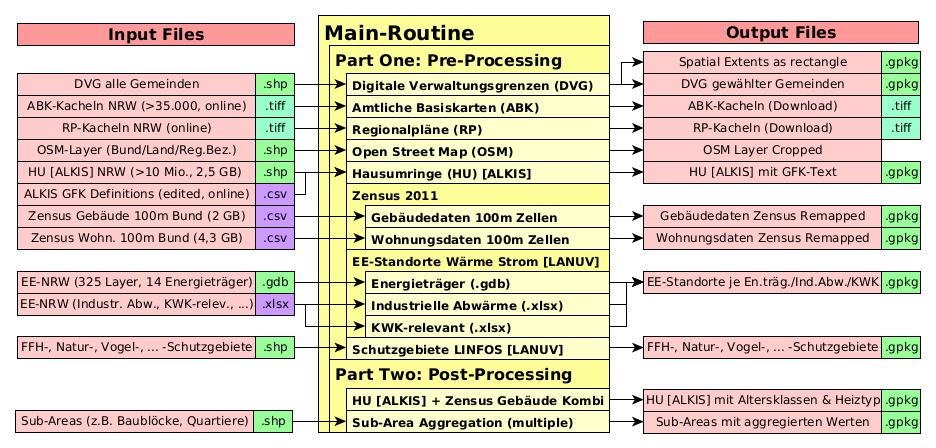
\includegraphics[width=\linewidth]{Medien/own/Softwarearchitektur_IO.png}
				\caption{Programm-Ablaufsplan mit In- und Output-Files je Datensatz inklusive Dateiformat}
				\label{fig:Code:Softwarearchitektur_IO}
		\end{figure}


	\section{Implementation: Teil I - Preprocessing}
		\label{sec:Code:Implementation1}
		
		Für jede der Datensatz-Bearbeitungs-Routinen im ersten Teil der Main-Routine wird das folgende Schema, teilweise in leicht abgewandelter Form, angewandt:\\
		\begin{itemize}
			\item \textbf{1) Check directory structure}, file- and folderpaths
				\subitem if necessary create folders
				\subitem if necessary download data and re-set filepaths
			\item \textbf{2) Load data} into pandas Dataframe or geopandas GeoDataframe
				\subitem crop to spatial extents of DVG selected or celllist (during loading)
				\subitem filter out layers/Merkmale or other things if filters are set (during loading)
			\item \textbf{3) Preprocess data} which might include:
				\subitem remapping of data (e.g. for Zensus data)
				\subitem adding geometry and convert to GeoDataframe
				\subitem translating attributes (e.g. GFK Code to GFK text for Hausumringe ALKIS data)
			\item \textbf{4) Write data} to file(s)
			\item \textbf{5) Preanalysis} (e.g. for Zensus data and Hausumringe ALKIS data)
			\item \textbf{6) Download QGIS Style-Definitionen} from Github Repository
		\end{itemize}
		
		Für die Bearbeitung jedes Datensatzes in Teil eins der Main-Routine ist für die räumliche Zurechtschneidung der Daten erforderlich, dass ein GeoDataframe mit den gewünschten räumlichen Maßen geladen wird. Im Laufe dieser Arbeit wurden hierfür die DVG gewählter Gemeinden verwendet, aus deren räumlicher Ausdehnung (Spatial Extents) ein Rechteck-Polygon zur Begrenzung und zugehörige Zellen-Listen für zellen-(/kachel-)basierter Datensätze abgeleitet wurden. 
		
		Für die meisten Datensätze ist die räumliche Zurechtschneidung im Code obligatorisch angesetzt, was die Nutzung des DVG-Datensatzes vorraussetzt (Dependancy). Alternativ ließe sich die Konstruktion eines Geodataframes zur räumlichen Abgrenzung auch anders bewerkstelligen. 
		
		Falls bereits präprozessierte Daten vorliegen, so werden diese in Schritt 2 geladen und Schritt 3 übersprungen. Für eine Nutzung in QGIS werden für manche Datensätze vorbereitete QGIS Styledefinitionen als .qml Dateien aus dem Github Repository des Python-Tools herunter geladen. Diese werden in QGIS automatisch beim Layer Laden mitgeladen, damit die Daten gleich korrekt dargestellt werden. 
				
		\subsection{GV-ISys}
		% Aufgabe 
		Der Dataframe wird verwendet, um Postleitzahlen oder Ortsnamen Geokoordinaten für den jeweiligen Ortsmittelpunkt zuordnen zu können. Dies wird bei der Aufbereitung der Daten aus dem LANUV-Datensatz für Energie-Erzeugungs-Anlagen Standorte NRW benötigt, s. \autoref{sec:Code:Implementation1:EENNRW}
		
		Das Sheet mit Liste aller politisch selbstständigen Gemeinden in Deutschland wird im Excel-File des GV-ISys Datensatzes wird in einen Pandas Dataframe eingelesen. Die 5 Headerzeilen werden aufgrund kombinierter Tabellen-Zellen ignoriert. Die Spalte mit Postleitzahlen wird als String eingelesen, damit vorangehende Nullen erhalten bleiben. Zum Referenzieren, werden die Variablen für Spaltennummern definiert, in denen sich die Segmente des ARS, die zugehörigen Gemeindenamen, Postleitzahlen, Längen- und Breitengrade finden.
		
		\subsection{Digitale Verwaltungsgrenzen (DVG)}
		\label{sec:Code:Implementation1:DVG}
%			Die Liste aller politisch selbstständigen Gemeinden in NRW (10.000+) aus dem GV-ISys wird genutzt, um bei Input einer Liste von Gemeindenamen z.B. ['Wuppertal','Solingen','Velbert'] eine Liste der zugehörigen AGS zu erhalten z.B. ['05124000','05122000','05158032']. \todo{GV-ISys bisher nicht genutzt}
			
			Die DVG werden genutzt, um später andere Datensätze räumlich zurecht zu schneiden. Für die Erstellung eines Geodataframes mit den DGV ausgewählter Gemeinden wird das shape file mit den DGV aller politischer Gemeinden NRWs ausgelesen und die Einträge anhand eines Abgleichs mit einer Liste mit Gemeindenamen oder einer Liste mit AGS gefiltert.
			
			Für die Filterung der Zensusdaten wird aus dem DVG-Geodataframe eine Liste mit Gitterzellen-IDs abgeleitet.
			Hierfür werden die bounds des DVG-Geodataframe, also die maximalen und minimalen X- und Y-Koordinaten ausgelesen. Aus diesen wird unter Angabe einer INSPIRE-kompatiblen Gitterzellen-Größe (z.B. '100m' oder '1km') die Liste mit Zellennamen erstellt. Die gelisteten Zellen decken im beim Zensusdatensatz verwendeten KBS (EPSG:3035) ein Rechteck ab, welches die DGV voll umfasst. Die Zellennamen-Konvention entspricht der Gitterzellen-ID-Konvention, welche auch im Zensus-Datensatz verwendet wird. 
			
			Für die Selektierung der passenden Raster-Files aus dem Datensatz für Regionalpläne und für Amtliche Basiskarten wird auf ähnliche Weise aus den Bounds des DVG-Geodataframe eine Liste mit passenden Kachel-Namen abgeleitet. 
			Die Regionalpläne (RP) liegen in 8x8 $km^2$ Kacheln, die Amtlichen Basiskarten (ABK) in 1x1 $km^2$ Kacheln vor. Für RP und ABK gilt KBS = EPSG:25832 \\
			
			Als Namenskonventionen gelten jeweils: \\
			Zensus: '<Einheit>N<y-Koordinate in \flq Einheit\frq>E<y-Koordinate in \flq Einheit\frq >\\
			RP: 'rp\_32<y-Koordinate in km>\_<x-Koordinate in km>\_8\_nw'\\
			ABK: 'abk\_32<y-Koordinate in km>\_<x-Koordinate in km>\_1'\\
			
			Die Liste aus Kachel- bzw. Zellennamen sieht dann bswp. wie folgt aus: \\
			Zensus (100 m): ['100mN31153E41077', '100mN31153E41078', '100mN31153E41079', ...] \\ 
			Zensus (1 km): ['1kmN3115E4107', '1kmN3115E4108', '1kmN3115E4109', ...]\\
			RP: ['rp\_32352\_5664\_8\_nw', 'rp\_32360\_5664\_8\_nw', 'rp\_32368\_5664\_8\_nw', ...]\\
			ABK: ['abk\_32352\_5664\_1', 'abk\_32353\_5664\_1', 'abk\_32354\_5664\_1', ...]\\
			
			Für die Filterung von Geodataframes anderer Datensätze wird aus den bounds ein rechteckiges Polygon mit der räumlichen Ausdehnung (engl. spatial extent) in Form eines Rechtecks in INSPIRE-kompatiblen Koordiantensystem EPSG:3035 (LAEA Europe) erstellt. 
			
			Nicht implementiert ist die Definition von Rand-Abständen vom Rechteck-Geodataframe zu den eigentlichen DVG. 
			
%				\begin{lstlisting}[language=Python, label=code:dvg_cells, caption={Python Minimal-Beispiel: DVG, Gitterzellen (Zensus, ABK, RP) und Spatial Extent},firstnumber=1234, emph={printf, schokostuecke}] 
%gdf_dvg_selected = get_dvg_geodataframe(gem_list,fp_shp_dvg)

%celllist_zensus = get_celllist_zensus(gdf_dvg_selected, 
%										INSPIRE_size)
%celllist_rp = get_celllist_rp(gdf_dvg_selected)
%celllist_abk = get_celllist_abk(gdf_dvg_selected)

%gdf_spatial_extent = get_gdf_spatial_extent(gdf_dvg_selected)

%			\end{lstlisting}
		\subsection{ABK}
			Die Amtlichen Basiskarten (ABK) werden durch das Python-Tool automatisch von \textit{OpenGeoData.NRW} heruntergeladen. Die Liste der Dateinamen aller Kacheln, welche das gewünschte Rechteck um die gewählten DVG abdeckt, entstammt der Subroutine für den DVG-Datensatz. 
			
			Da das Einladen von mehr als 800 einzelnen Raster-Dateien in QGIS nicht möglich ist, wurde zusätzlich ein Bash-Script geschrieben, um die einzelnen .tif-Dateien zusammen zufügen. Das Bash-Script nutzt die Command-Line-Tools \textit{gdalwarp} und \textit{gdalbuildvrt}. Ersteres wird verwendet, um die Georeferenzierung der .tif-Dateien von Ground Control Points (GCP) zu einer geoaffinen Georeferenzierung zu ändern. Diese Art der Georeferenzierung wird benötigt, damit im zweiten Schritt mit \textit{gdalbuildvrt} alle einzelnen .tif-Dateien zu einem Mosaik in Form einer einzigen .vrt-Datei zusammengefügt werden können. 
			
			Ein automatischer Aufruf des Tools ist nicht implementiert, aber ein Hinweis auf eine manuelle Ausführung nach Verwendung des python-Tools wird bei einer ABK-Anzahl von 400 und größer ausgegeben.
			
			
		\subsection{OSM}
			Jedes der 18 Layer der OSM-Daten wird einzeln eingelesen, zugeschnitten und abgespeichert. Der Zuschnitt erfolgt direkt beim Einlesen auf die bounds der gewählten DVG (Rechteck) und als Speicherformat wird standardmäßig Geopackage verwendet, optional auch Shape-File. 
			
			Zur bequemen out-of-the-box Nutzung der OSM-Daten in QGIS werden Style-Definitionen mit dem Python-Tool automatisch aus dem eigenen Github-Repository in den Ordner der zugeschnittenen OSM-Daten geladen. Beim Laden der Layer in QGIS werden die Styles automatisch mitgeladen. Hierfür sorgt die Gleichbenennung der Style-Definitionen im .qml-Format gemäß der OSM-Layer-Bezeichnung. \cite{web_github_repo_code}
						
			Die eigenen Style-Definitionen basieren größtenteils auf denen von champs-libres aus dem Jahr 2020 \cite{web_gitlab_champs_libres}. Es wurden lediglich leichte Veränderungen vorgenommen. Beispielsweise wurde die Kolorierung einiger Objekte wie Gebäude, verkehrsrelevante Infrastrukturelemente wie Parkgebäude und -flächen sowie Flächen von Points of Interest angepasst. Zudem wurden in der aktuellen QGIS-Version nicht darstellbare Symbole im SVG-Format (Scalable Vector Graphic) ersetzt. Zu den verwendeten Symbolen gehören unter Anderem gekreuzte Hämmer für Tagebaue, Baumsymbole für Waldflächen und Sterne für Friedhöfe als religionsunspezifisches Repräsentationssymbol. Die Anpassung der Styledefinitionen wurde manuell in QGIS umgesetzt. 
			
		\subsection{Hausumringe [ALKIS]}
			% 1) Aufgabe: Einlesen, Cropping, GFK-Spalte in textform
			Um die Hausumringe aus dem ALKIS inklusive leserlicher Bezeichnung der Gebäudefunktion (GFK) darzustellen, werden diese in einen Geodataframe gelesen und um eine Spalte mit GFK in Textform erweitert. 
			
			% 2a) Umsetzung: Einlesen, Cropping
			Beim Einlesen wird der Geodataframe direkt mittels \textit{fiona} auf die boundbox aus der räumlichen Ausdehnung der DVGs zugeschnitten. Mit dem gegebenen Setup dauerte das Einlesen inkl. Cropping für die Gemeinden Wuppertal, Velbert und Solingen auf diese Weise ca. 70 Sekunden. Das Einlesen des gesamten Shapefiles ohne Zuschneiden dauerte zum Vergleich über 15 min und nahm ca. 14 GB Arbeitsspeicher in Anspruch. Nachträgliches Cropping erwies sich zusätzlich zur langen Bearbeitungsdauer auch als ungeeignet, da während des Zuschneidens der Arbeitsspeicher von 16 GB und Swapfile von 16 GB überladen wurde. 
			
			% 2b) Umsetzung: Übersetzung
			Für die Übersetzung von GFK-Code zu GFK-Text wird die .csv-Datei mit GFK-Definitionen aus dem Github-Repository des Tools in einen pandas Dataframe gelesen. Im Anschluss werden die Codes der GFK-Spalte des Geodataframes in Textform übersetzt, dies geschieht vektorwertig mit der Funktion \textit{.apply()}. 
			
			Die .csv-Datei wurde ursprünglich aus der .xml-Datei mit Definitionen aller ALKIS-Gebäude- und Bauwerksunktionen aus dem ALKIS-Repository abgeleitet. Da die xml-Defnitionen sehr verschachtelt aufgebaut sind, wurde der ursprüngliche Code zum Extrahieren der GFK-Defnitionen zur Erstellung eines GFK-Übersetzungs-Dataframes beibehalten. 
			
			% 3) Schreiben
			Zum Schluss wird der Geodataframe als GeoPackage und optinal als Shapefile gespeichert.\\
			
			\textbf{Minimalbeispiel:}\\
			\autoref{code:hu_gfk} zeigt ein Minimal-Code-Beispiel des entwickelten Software-Tool, in der beide Versionen zur Übersetzung der GFK-Codes mit originärer .xml-Datei (original version) und manuell modifizierter .csv-Datei (later version) gezeigt werden. Die Daten werden geladen, dabei zugeschnitten, die GFK-Codes übersetzt in GFK-Texte und die Datei als Geopackage (.gpkg) gespeichert. 
			
			\begin{lstlisting}[language=Python, label=code:hu_gfk, caption={Python Minimal-Beispiel: Präprozessierung Hausumringe Datensatz},firstnumber=1234, emph={printf, schokostuecke}] 
gdf_hu = gpd.read_file(fp_hu_shp_raw,
								bbox=gdf_spatial_extent,engine="fiona")
#hu_dict_df = get_hu_dict_df(fp_hu_gfk_xml) # oiginal version
hu_dict_df = pd.read_csv(fp_hu_gfk_mod_csv, 
								encoding='unicode_escape') # later vers.
gdf_hu['GFK_text'] = gdf_hu['GFK'] # add column for GFK-Text
gdf_hu['GFK_text'] = gdf_hu['GFK_text'].apply(gfk_code_to_text)
gdf_hu.to_file(fp_hu_gpkg_crop,driver='GPKG')
			\end{lstlisting}
			
			\textbf{Anmerkung zur GFK-Code zu GFK-Text Übersetzung:}\\
			Die Methode \textit{gfk\_code\_to\_text} wurde 'quick and dirty' geschrieben und ist 'bad practice', da sie auf der Verwendung globaler Variablen beruht (\textit{hu\_dict\_df}). Die \textit{.apply()} Funktion zur Übersetzung in einem sauberen Ansatz mit Pythons Lambda Funktion unter Verwendung mehrerer Argumente zu verwenden (\textit{row}, \textit{hu\_dict\_df}) gelang nicht ohne weiteres, weshalb die Methode so belassen wurde.  
			
			%Im Anschluss wird dem Geodataframe eine neue Spalte für die GFK-Texte hinzugefügt, initial mit den GFK-Codes als Werten. Mit der Funktion .apply werden diese Code-Werte unter Verwendung des Übersetzungs-Dataframes in GFK-Texte umgewandelt. 
			

			%Der Geodataframe wird zum Schluss einmal als Shape File und einmal als GeoPackage gespeichert. Für die ca. 500.000 Hausumringe-GDF innerhalb der DVG von Wuppertal, Velbert, Solingen dauerte der Schreibprozess für das Shape File ca 163 Sekunden, für das GeoPackage ca. 87 Sekunden.
		\subsection{Raumwärme-Bedarfsmodell [LANUV]}
			Die Raumwärme-Bedarfsmodell liegen sowohl als über 1~GB großes komprimiertes Shape-File für ganz NRW vor als auch in Form von einzelnen komprimierten Shape-Files je Gemeinde in NRW. Um Speicherplatz zu sparen, werden nur die Rohdateien aller nötiger Gemeinden herunter geladen. 
			
			Aus den DVG aller Gemeinden NRWs wird abgeleitet, welche Gemeinden innerhalb der Boundbox (Rechteck) um die ausgewählten Gemeinden liegen. Für die ausgewählten Gemeinden Wuppertal, Velbert und Haan, umfasst die erstellte Liste beispielsweise 26 Gemeinden u.a. Remscheid, Schwelm und weitere direkt umliegende Gemeinden. Es werden eine Liste mit den Gemeindenamen abgeleitet und eine zweite Liste mit den AGS der jeweiligen Gemeinden. Aus diesen beiden Listen werden die URL's der herunter zu ladenden komprimierten Shape-Files von \textit{OpenGeoData.NRW} abgeleitet. Die Gemeindenamen werden entsprechend angepasst, durch Abschneiden gewisser Zeichenketten und Änderung von Umlauten in Vokalkombinationen oder "ß" in "sz". 
			
			Die Daten werden initial heruntergeladen, entpackt, in Geodataframes geladen, kombiniert, auf die erwähnte Boundbox (RechtecK) zugeschnitten und abgespeichert. Falls bereits präprozessierte und zugeschnittene in dieser Form vorliegen, werden diese geladen, statt den Prozess erneut durchzuführen. Sowohl Download als auch Entpacken als auch einzeln Laden und Zusammenfügen werden nur durchgeführt, falls die Daten nicht in der letzt-möglich präprozessierten Form vorliegen.
			
			
		\subsection{Zensus 2011}
			% Aufgabe
			Da der Zensus-Datensatz das gesamte Bundesgebiet umfasst und diverse Merkmale abdeckt von denen nur ein Teil für Wärmeplanungen relevant ist, soll der Datensatz eingelesen und auf eine gewünschte Region und prädefinierte Merkmale reduziert werden. Des weiteren soll der Datensatz auf Datenlücken untersucht werden. Wenn möglich, sollen diese kenntlich gemacht und im Idealfall aufgefüllt werden. Zum Schluss soll der Datensatz in ein QGIS-kompatibles Format exportiert werden. 
			
			\subsubsection{Zensus 2011 - Ansatz}
				% Ansatz Inhalt: Formatieren
				Für eine einfache Nutzung in QGIS und zur leichteren späteren Verwendung mit anderen Datensätzen zusammen werden die Daten des Zensus stark pre-prozessiert. Hierfür wird ein neues Tabellen-Format gewählt, in welcher jeder Gitterzelle nur eine einzelne Zeile spalte zugewiesen wird und die Anzahl erfasster Merkmals-Ausprägungen (z.B. Anzahl der Wohnungen mit Baualtersklasse von 19xx bis 19xx) in unterschiedlichen Spalten hinterlegt wird.
			
				% Ansatz Code: Objektorientiert inkl. Docstrings
				Für dieses aufwendigere Pre-Proezessieren wird für den Zensus-Datensatz ein objektorientierter Ansatz gewählt, indem die Klasse \textit{zensusdata} definiert wird. Die Klasse ist mit einem \textit{\_\_docstring\_\_} versehen, in welchem Attribute und Methoden erläutert werden. Dieser kann wie in \autoref{fig:help_zensusdata} gezeigt mit \textit{help(zensusdata)} innerhalb von Python abgerufen werden, zudem werden die Docstrings in gängigen IDEs bei Verwendung von Klassen und Methoden auch automatisch mit angezeigt. 
				
				% Klassen-Beschreibung, Attribute --> Verschieben nach Umsetzung
				Die Klasse \textit{zensusdata} beinhaltet als Attribute unter anderem den Filepath zu den Rohdaten, optional eine Liste mit Gitterzellen-ID's zum Zurechtschneiden, eine Liste zur Spalten-Referenzierung (z.B. identifier = 'Gitter\_ID\_100m', key1 = 'Merkmal', key2 = 'Ausprägung\_Text, value = 'Anzahl'], ein Merkmals-Dictionary mit allen dem jeweiligen Merkmal zugehörigen Ausprägungen, eine Liste von Merkmalen, nach denen gefiltert wird, einen pandas dataframe mit orginalem Format, einen pandas data frame mit neuem Zeilen-/Spalten-Format und einen geodataframe mit der neuen Formatierung zum Bearbeiten innerhalb von Python.
			
			\subsubsection{Zensus 2011 - Programmablauf}
				% Programm Ablauf 
				% 1) Daten einlesen und reduzieren auf Zellen und Merkmale
				\textbf{Daten einlesen und reduzieren:}\\
				Zu Beginn wird der gesamte Zensusdatensatz aus der csv-Datei in einen Pandas Dataframe geladen. Danach wird dieser mittels zwei Listen räumlich auf alle gewünschten Gitterzellen und auf alle zu untersuchenden Merkmale reduziert. Die Liste der Gitterzellen-IDs wird aus den Datensatz der DVG abgeleitet, s. \autoref{sec:Code:Implementation1:DVG}, die Liste, welche als Merkmalsfilter dient, wird vorher definiert und beinhaltet default-mäßig die Baualtersklasse ('BAUJAHR\_MZ') und den Heiztyp ('Heiztyp').  \\
				
				% todo code:
				% celllist_zensus_appear
				% df erstellen
				% mit apply füllen (dynamisch je nach m_filter)
				% sollte schneller funktionieren als iterieren
				
				% 2) Daten remappen inkl. Merkmalsfilter und Qualitätsfilter
				\textbf{Daten reformatieren (Remapping):}\\
				Um die Daten später in QGIS nutzen zu können, werden die Daten im Anschluss formatiert und hierfür in einen neuen Dataframe remapped. Alle Zeileneinträge gleicher Gitterzellen werden in eine einzelne Zeilen des neuen Dataframe übertragen, wobei die Werte der Anzahl einer jeweiligen Merkmals-Ausprägung im neuen Dataframe jeweils einer neuen Spalte zugewiesen wird. 
				
				Es werden nur Spalten für Merkmale erstellt, nach denen auch mittels Merkmals-Filter beim Einlesen bereits gefiltert wurde. Die Bezeichnung dieser Spalten im neuen Dataframe werden einem Merkmals-Dictionary entnommen. Optional lassen sich in diesem Schritt bereits Merkmals-Ausprägungen zusammenfassen (z.b. zwei verschiedene Baualtersklassen), indem im Dictionary für mehrere Merkmals-Ausprägungen die gleiche neue Spaltenbezeichnung verwendet wird. Die Einzelwerte werden dann summiert. In \autoref{fig:help_zensusdata.remap_zensusdata} ist die Ausgabe des Docstrings für die entwickelte Methode zum Remapping in Python gezeigt. \\
				
				%Die Werte sind zwar numerisch, werden aber zur besseren Kennzeichnung von Nicht-Werten als Strings hinterlegt. Null-Werte werden mit dem String \textit{00} gekennzeichnet. \todo{check}
							
				\textbf{Qualitäts-Check beim Remapping}:\\
				Je nach gewähltem Qualitäts-Schwellenwert (\textit{zensus\_q\_thresshold} = 0, 1 oder 2) werden beim Remapping nur Werte berücksichtigt, deren Datenqualität (Spalte \textit{Anzahl\_q}) dem Schwellenwert oder kleiner entsprechen. 0 steht für \frqq keine bis nur geringe\flqq, 1 für \frqq starke\flqq und 2 für \frqq inakzeptabele\flqq Abweichung nach Zensus-Maßstäben. 
				Zusätzlich werden zwei gesonderte Spalten für jedes gewünschte Merkmal hinzugefügt. Hier werden alle Einzelwerte der jeweiligen Gitterzelle deren Datenqualität den Wert 1 bzw. 2 besitzen summiert. Dies dient der Anzeige wie groß der Anteil an Daten mit Datenqualität 1 oder 2 in einer jeweiligen Gitterzelle für das entsprechende Merkmal ist. \\ 
					
				% 3) Datenlücken erkennen: Spalte Diff = Spalte INSGESAMT minus Summe anderer Spalten
				\textbf{Datenlücken erkennen und kenntlich machen:}\\
				Zur Kenntlichmachung von Datenlücken werden zwei weitere Spalten hinzugefügt. In diese wird die absolute und relative Differenz angegeben von der gesamten Anzahl aller Gebäude bzw. Wohnungen der Gitterzelle und der Summe der Gebäude bzw. Wohnungen die mit Merkmal (entsprechend dem jeweiligen Q-Schwellenwert) erfasst wurden. 
				
				Hinweis: Wird der Zensus-Datensatz für Gebäude verwendet, können die Daten auch mit den offiziellen Hausumringen (HU) aus dem ALKIS abgeglichen werden, indem die Anzahl aller \textit{Centroids} von HUen mit der im Zensus-Datensatz angegebenen Gesamtzahl an Gebäuden in der selben Gitterzelle abgeglichen werden.\\
				
				\textbf{Merkmals-Dictionary:}\\
				Das Merkmals-Dictionary beinhaltet alle Merkmale als Keys. Für jedes Merkmal ist eine Liste mit Tuplen hinterlegt, wobei für jede Ausprägung ein Tuple enthalten ist. Diese Tuple enthalten die drei Einträge für den Zensus-Ausprägungs-Code, den Zensus-Ausprägungs-Text und die zugehörige neue Spaltenbezeichnung für das Remapping. Die letzten vier Einträge in der Liste für jedes Merkmal sind reserviert und enthalten Tuple für die Qualitäts-Spalten und Differenz-Spalten. Für das Merkmal 'BAUJAHR\_MZ' sieht die Liste bspw. wie folgt aus:  
				$\left[$('1','Vor 1919','BauVor1919'),
				('2','1919 - 1948','Bau1919\_48'),
				... ,
				('10','2009 und später','BauNac2008'),
				('','q1','Q1Baujahr'),
				('','q2','Q2Baujahr'),
				('','Diff\_abs','DiffAbsAlt'),
				('','Diff\_rel','DiffRelAlt').$\right]$
				
				Anmerkung: Als Standardeinstellungen werden allen Merkmals-Ausprägungen individuelle neue Spaltenbezeichnungen zugewiesen, die kleiner gleich 10 Zeichen lang sind, da diese sonst bei einem Shapefile-Export abgeschnitten würden. \\
				
				% 4) Daten ableiten: Dämmpotential-Abschätzung
				\textbf{Daten ableiten: Dämmpotential-Abschätzung}\\
				Ein einfaches Modell zur Estimierung des Dämmpotentials wurde überlegt, aber nicht implementiert, aufgrund der Schwierigkeiten auf die Schnelle ein geeignetes tragfähiges Modell zu entwickeln.
									
				Die Zensus-Daten in remappierter Form bieten allerdings eine gute Form, um ein solches Modell einfach in Python oder QGIS zu implementiert. Ein einfaches Berechnungsmodell könnte z.B. wie folgt aussehen: \\
				
				$Dämm_{potential} = \left[\sum_i^{N_{alt}} (n_{alt,i}} \cdot g_{alt,i})\right] \cdot A_{ges} = \left[\sum_i^{N_{alt}} (n_{alt,i}} \cdot g_{alt,i})\right] \cdot \left[\sum_j^{N_{fläche}}
			(n_{fläche,j} \cdot A_{fläche,j})\right] $\\
				 
				Wobei $N_{alt}$ die Anzahl verschiedener Altersklassen ist, $n_{alt,i}$ die Anzahl an Wohnungen der Altersklasse $i$ in der jeweiligen Gitterzelle ist, $g_{alt,i}$ der Gewichtsfaktor mit dem Wohnungen der jeweiligen Altersklasse berücksichtigt werden sollen, $N_{fläche}$ die Anzahl verschiedener Wohnungsgrößenklassen und $n_{fläche,j}$ die Anzahl der Wohnungen der Wohnungsgrößenklasse $j$ in der jeweiligen Gitterzelle ist und $A_{fläche,i}$ die Fläche mit der die jeweilige Wohnungsgrößenklasse berücksichtigt werden soll. Unberücksichtigt bei diesem Modell wäre Leerstand. Die unterschiedlichen Durschnittsgrößen von Wohnungen verschiedener Altersklassen könnten im Gewichtungsfaktor mit berücksichtigt werden.\\ 
				
				% 5) Geometrie Daten hinzufügen % 6) Speichern
				\textbf{Geometriedaten hinzufügen und Speicherformate:}\\
				Zum Schluss wird dem Dataframe eine Geometriespalte hinzugefügt in welcher die Polygone der Gitterzellen abgeleitet aus der Gitterzellen-ID in WKT-Format eingetragen werden. Der Dataframe kann direkt als .csv-Datei gespeichert werden oder zu einem geopandas GeoDataframe konvertiert und als ESRI Shapefile und/oder als OGC GeoPackage gespeichert werden.\\
				
				% 6) Pre-Analyse
				\textbf{Pre-Analyse-Routine:}\\
				Zu Analysezwecken wird im stdout die Summe der Q1-, Q2- und DiffAbs-Spalten angegeben sowie der Mittelwert der DiffRel-Spalte. Negative und Positive Werte werden nicht seperat berücksichtigt. Zusätzlich werden für jedes Merkmal im Merkmalsfilter Dataframes erstellt, in welcher die Gesamtzahl aller Einheiten (Wohnungen oder Gebäude) je Merkmals-Ausprägung absolut und relativ zur Gesamtzahl an Einheiten gelistet sind. Ebenso enthalten sind die Summen für alle Einheiten mit Merkmal, ohne Merkmal und insgesamt. Die Infos werden dem remapped Dataframe entnommen, dementsprechend werden nur Werte entsprechend dem Qualitäts-Schwellenwert berücksichtigt. Dies wird beim Speichern mit 'q0', 'q1' oder 'q2' im Dateinamen gekennzeichnet. 
				
				% Zusätzliche Info im Stdout zu Q1, Q2, DiffAbs Summen und DiffRel Mittelwert ...
				
		\subsection{Energie-Erzeugungs-Anlagen Standorte NRW [LANUV]}
		\label{sec:Code:Implementation1:EENNRW}
			% Aufgabe
			% Programm Ablauf 
			% 1) Daten einlesen und reduzieren auf DGV
			Um Vektordaten von Standorten für alle Energieträger aus der Geodatabase und zusätzlich für Industrielle Abwärme und KWK-relevante Anlagen aus der Excel-Datei auszulesen, gegebenenfalls mit Geometriedaten zu versehen (Excel-Datensatz) und abzuspeichern wurden die folgenden Schritte im Code implementiert.\\
			
			\textbf{Layerweise Vorgehen bei der Geodatabase:}\\
			% Format
			Da die Geodatabase über 325 Layer verfügt und jeder Geopandas GeoDataframe (GDF) nach Definition nur über ein Layer je GDF verfügt, wird jedes Layer seperat als GDF in einem gemeinsamen Dictionary hinterlegt mit dem jeweiligen Layernamen als Key. 
			
			% Layernamen-Filterung (Black- und Whitelist) + Zurechtschneiden auf Spatial Extents
			Zur Layer-Filterung wurde die Option einer Black- und einer Whitelist implementiert. Der Layername vor Einlesen mit beiden Filterlisten verglichen und das Layer gegebenenfalls übersprungen. Im Anschluss werden potentielle Tippfehler im Layernamen korrigiert, um diese zu vereinheitlichen. ('Windbetrieb' zu 'WindBetrieb' und 'Planungsreg' zu 'PlanungsReg', da hier beide Schreibweisen auftauchten.) Beim Einlesen des jeweiligen Layers wird der GDF bereits auf die Spatial Extents der gewählten DVG zugeschnitten (Rechteck). 
			
			% Speicherformat Geopackage - Nicht implementiert Shapefile und Geodatabase
			Als Speicherformat für die zurechtgeschnittenen Layer wurde OGC GeoPackage gewählt. Eine optionale Schreiboption für Shapefiles wurde zu Beginn implementiert, aber auskommentiert. Hierfür wurden Attributeswerte mit dType 'Datetime' zu 'Strings' konvertiert und alle 'ß' in Attributsnamen zu 'B'. Viele der insgesamt 75 in allen Layern zusammen genommenen auftretenden Spaltenbezeichnungne verfügen allerdings über mehr als 10 Zeichen (Shape-File-Limitierung), was für Geopackages kein Problem darstellt. Von einer Speicherung als Geodatabase wird ebenso abgesehen. Diese wäre auch nicht ohne weiteres möglich, da der offene GDAL Treiber für Geodatabase nur über Lese-, nicht jedoch über Schreibfunktionen verfügt. \\
			
			\textbf{Sheetweise Vorgehen bei Excel-Datei (Industrielle Abwärme, KWK):}\\
			Um die Daten zu Standorten mit industrieller Abwärme und KWK-Relevanz aus der Excel-Datei einzulesen und in ein GeoPackage zu übertragen, werden die beiden Sheets zunächst in zwei Pandas Dataframes eingelesen. Beiden Dataframes wird eine Spalte mit Geometriedaten hinzugefügt. Für den Industrielle Abwärme Dataframe werden die x- und y-Koordinaten direkt aus dem Dataframe ausgelesen, für den KWK Dataframe wird die PLZ oder der Ortsname verwendet, da keine Geo-Koordinaten gegeben sind.
			
			% 2) Daten speichern
			Beide Dataframes werden zu Geodataframes konvertiert, das KBS zu EPSG:25832 angepasst, auf die Spatial Extents der gewählten DVG zugeschnitten (Rechteck) und als Geopackage gespeichert.  \\
			
			% 3) Additional Info
			\textbf{Geometrie-Daten aus PLZ für KWK-Standorte:}\\
			Um die Geometriedaten für die Ortsmittelpunkte im KWK Dataframe zu bestimmen, wird über alle 587 der unikal auftretenden PLZ von insgesamt 1601 Einträgen iteriert. (Wenn PLZ mehrfach auftreten, wird nur einmal über diese iteriert.) Die Koordinaten der meisten PLZ werden mit der Python-Library \textit{pgeocode} ermittelt (575), die übrigen, für welche dieser Ansatz nicht funktionierte, mit der etwas langsamer arbeitenden Python-Library \textit{geopy} (12). Beide Librarys nutzen die PLZ und geben die Koordinaten im KBS EPSG:4326 (WGS84) aus. 
			
			Als Fall-Back-Alternativen falls diese Libraries nicht funktionieren sollten, wurden zwei eigene Methoden im Script hinterlassen. Die erste überprüft, ob die PLZ im GV-ISys Datensatz auftaucht, die zweite, ob der Ortsname <ort> direkt oder in abgewandelter Form in exakt dieser Schreibweise im GV-ISys Datensatz auftaucht. ('<ort>', '<ort>, Stadt', '<ort>, Hansestadt') notfalls ob es Gemeindenamen gibt, die den Ortsnamen überhaupt enthalten. Beide Methoden beachten Groß- und Kleinschreibung und lesen bei Fund aus diesem die Koordinaten im KBS EPSG:4326 (WGS84) ab. 
			
			Hinterlassen werden diese, um unerwartete Exponate bei Ortsnamen abzufangen, wobei die zuletzt beschriebene Methode gegebenenfalls zu falschen Ergebnissen führen könnte, da beispiels
			Methode c) fand beispielsweise für die PLZ 41538 Anwendung, für die Ortsnamen teils mit 'Dormagen' und teils mit 'DORMAGEN' angegeben waren.

			\autoref{fig:code:ee_nrw:sdout} zeigt den Stdout beim Ausführen des Python-Tools für diesen Datensatz mit der Default White- und Blacklist.\\
			
			\begin{figure}[h]
				\centering
				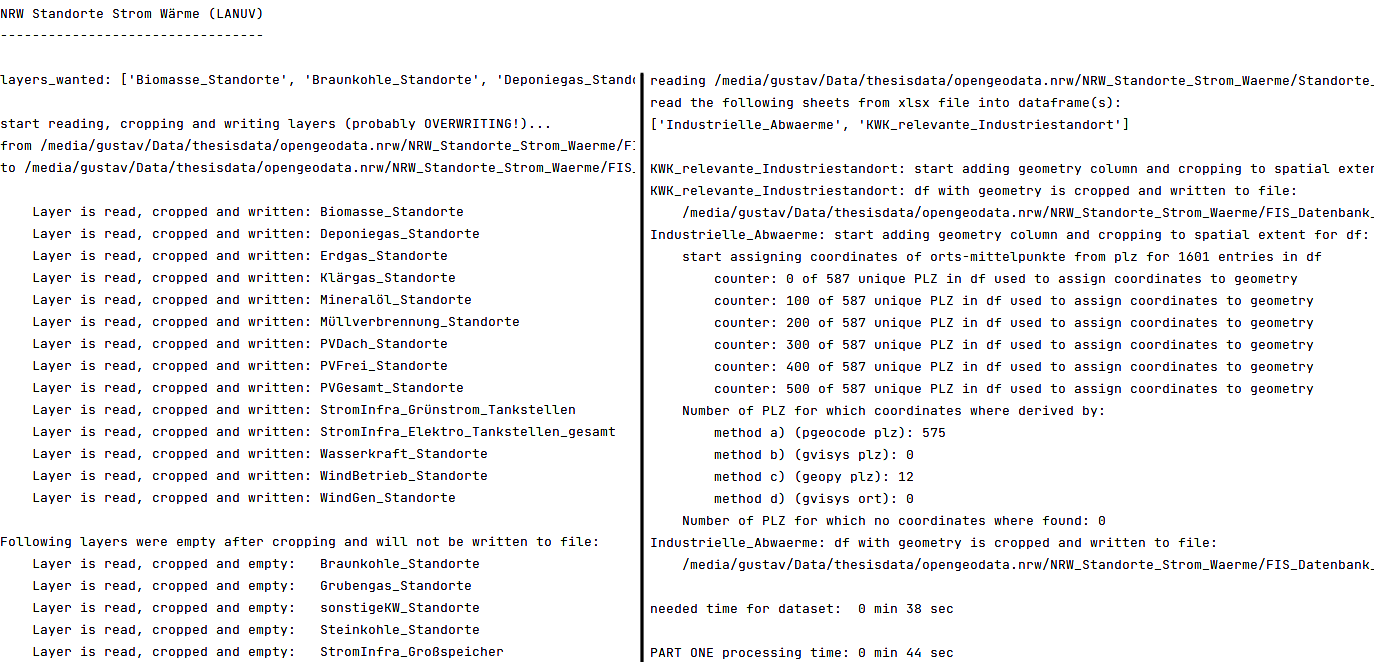
\includegraphics[width=\linewidth]{./Medien/own/ee_nrw/ee_nrw_sdout.png}
				\caption{Stdout Präprozessierungs-Routine für den Erzeugungs-Anlagen NRW Datensatz des LANUV}
				\label{fig:code:ee_nrw:sdout}
			\end{figure}
			
			\textbf{Nachtrag:} Die genauen x- und y-Koordinaten in ETRS89/UTM32 (EPSG:25832) liegen auch im Datensatz für Industrielle Abwärme Standorte vor und sind mit den Bezeichnungen Rechtswert und Hochwert benannt. Die Georeferenzierung wurde korrigiert und wird in der aktuellen Version des Python-Tools aus diesen Koordinaten abgeleitet. Aus Zeitgründen wurden dieses Unterkapitel und \autoref{fig:code:ee_nrw:sdout} nicht mehr korrigiert. 
			
			
		\subsection{Schutzgebiete Landschaftsinformationssammlung (LINFOS) [LANUV]}	
			Es können alle in der Landschaftsinformationssammlung (LINFOS) vom LANUV gesammelten Datensätze verschiedener Arten von Schutzgebieten vollständig automatisiert heruntergeladen, entpackt, von Shape-Files in Geodataframes geladen, räumlich zugeschnitten und als Geopackages abgespeichert werden. 
			
			
	\section{Implementation: Teil II - Postprocessing}
	\label{sec:Code:Implementation2}
			
			
		\subsection{Kombination von Hausumringen [ALKIS] und \\Gebäude-Merkmalen [Zensus]}
		\label{sec:Code:Implementation2:HU_Alkis_Zensus_Merkmalszuweisung}
			% Intro: Idee - Darstellung von Altersklassenverteilung in Gebiet
			Die Idee ist Hausumringen aus dem ALKIS Datensatz Ausprägungen von Merkmals-Ausprägungen aus dem Zensus-Gebäude-Datensatz zuzuordnen. Dies dient anschaulicheren Darstellungs-Möglichkeiten in GIS, in diesem Fall für die Darstellung der Baualtersklasse von Gebäuden, um das energetische Modernisierungspotential visuell abschätzen zu können.
					
			% Beschreibung: Problem - Darstellung von Zensusdaten & Lösung
			Mit den Zensus-Datensätzen (remapped) für Wohnungen und Gebäuden lässt sich in jeder Gitterzelle immer nur jeweils ein Attribut (z.B. Anzahl einer bestimmten Baualtersklasse wie 'BauVor1919') gleichzeitg übersichtlich darstellen, z.B. durch semi-transparente Einfärbung der Gitterzellen. Gegebenenfalls können noch ein, zwei weitere Attribute zusätzlich dargestellt werden, z.B. durch Einfärbung von darübergelegten Punkt- oder Linienmustern. Diese Darstellungsform eignet sich nicht zur simultanen Darstellung einer Vielzahl von Attributen. Die Zuordnung von Altersklassen aus den Zensus Gebäudedaten zu Hausumringen löst dieses Problem.\\

			\textbf{Hausumringe: GFK-Einordnung}\\
			Eine Zuweisung soll nur durchgeführt werden für Hausumringe, deren Bauwerks- und Gebäudefunktion (GFK) indiziert, dass diese auch als Gebäude in der Zensus-Datenerhebung mit erfasst wurden. Hierzu gehören alle GFK mit Wohnzweck.
			
			Die Einordnung der GFK nach Wohnzweck wurde adhoc entschieden und manuell tabellarisch zugeordnet. Die verwendete Tabelle mit ALKIS GFK-Code und GFK-Text Definitionen, wurde aus der .xml Datei von ALKIS extrahiert, als .csv-Datei gespeichert, manuell modifiziert und im Github-Repository für diese Thesis geladen. Das Python-Tool lädt bei Bedarf die .csv mit Definitionen aus dem Repository. \cite{web_github_repo_code} 
			
			Da zunächst fälschlicherweise davon ausgegangen wurde, dass auch Nichtwohngebäude (NWG) in den Zensusdaten erfasst wurden, wurde zuvor eine Einordnung der GFK nach Altersklassen-Relevanz vorgenommen. Diese Zuordnung für GFK von Wohn- und NWG wurde in einer seperaten Spalte 'alt\_rel' in der .csv-Datei eingefügt und zu Analysezwecken beibehalten. 
			
			Als altersklassen-relevant wurden hierbei unter anderem GFK eingestuft aus dem Bereich Wohnen, GHD, Bildungs- und Forschungseinrichtungen, soziale Einrichtungen und Gebäude für öffentliche Zwecke. Als irrelevant wurden unter anderem GFK eingestuft wie Garagen, Schuppen, Überdachungen, Messe- oder Fabrikhallen, Burgen, Schlösser, Mauern. \\
			
			% Beschreibung: Umsetzung - Teil 1: Gitterzellen-Zuordnung
			\textbf{Hausumringe: Gitterzellen-Zuordnung}\\
			Für die Umsetzung wird im ersten Schritt zunächst die Zuordnung von Hausumringen zu Gitterzellen vorgenommen. Hierfür wird aus dem jeweiligen Polygon eines jeden Hausumrings der Centroid, also der jeweilige Flächenschwerpunkt bestimmt und als Attribut hinzugefügt. Aus den Koordinaten des Centroid wird nach deren Projektion ins KBS der Zensusdaten (EPSG:3035) die zugehörige Gitterzelle identifiziert und die Gitterzellen-ID als Attribut hinzugefügt. Das Hinzufügen der Attribute Centroid und Gitterzellen-ID wird vektoriell für den gesamten Geodataframe der Hausumringe umgesetzt. Mit dem entwickelten Python-Tool und der gegebenen Hardware dauert die Bestimmung der Centroids ungefähr 1 min und die Bestimmung der Gitterzellen-ID ungefähr 10 Sekunden für ca. 500.000 Hausumringe (Solingen, Velbert, Wuppertal). \\
			
			
			\textbf{Hausumringe: Merkmals-Zuweisung aus Zensus Gebäude-Datensatz}\\
			Für die Zuweisung von Zensus Merkmals-Ausprägungen wird für jedes zuzuweisende Merkmal ein gleichnamiges Attribut im HU GDF hinzugefügt (neue Spalte), welches gleich dem zuzuweisenden Merkmal benannt ist. (z.B. 'BAUJAHR\_MZ' für Baualtersklassen oder 'Heiztyp' für die Heizungsform). Die Spalten sind zunächst mit dem Default-Wert 'Unbekannt' gefüllt. 
			
			Die Zuweisung der aus dem Zensus Gebäude-Datensatz entnommenen Werte wird iterativ für jede Gitterzelle mit Hausumringen durchgeführt. Gibt es keine korrespondierende Zelle im Zensus Gebäude-Datensatz, wird die jeweilige Zelle übersprungen. Andernfalls wird über alle zuzuweisenden Merkmale iteriert und für jedes Merkmal ($merk,i$) wie folgt vorgegangen. 
			
			Zunächst wird eine Liste $list_{zensus,merk,i,ausp,count}$ erstellt, in welcher die Anzahlen von Gebäuden einer jeden Merkmals-Ausprägung ($ausp$) nach Zensus Gebäude-Datensatz gelistet werden. (z.B [0,3,0,3,0,0,0,0,0,0,0] bei zehn Ausprägungen ($N_{merk,i,ausp} = 10$) mit den angegebenen Häufigkeiten in der Gitterzelle)
			
			Damit die Zuweisung von Merkmals-Ausprägungen zu Hausumringen zumindest zellenweise vektorwertig durchgeführt werden kann, soll daraus eine Liste $list_{hu,merk,i,values}$ abgeleitet werden, in welche die jeweiligen zuzuweisenden Attributswerte im Hausumringe GDF gelistet sind. (z.B. $\left[$'Bau1919\_48','Bau1919\_48','Bau1919\_48','Bau1979\_86','Bau1979\_86','Bau1979\_86'$\right]$ für das Attribut 'BAUJAHR\_MZ') Die Länge von $list_{hu,merk,i,values}$ muss dafür der Anzahl an Hausumringen entsprechen, denen Werten zugewiesen werden sollen. 
			
			Für die Erstellung dieser Attributs-Werte Liste für die Hausumringe wird gemäß der folgenden Fallunterscheidung vorgegangen und die jeweils beschriebene Strategie gewählt, wobei $N_{geb,merk,i} = \sum_j^{N_{merk,i,ausp}}n_{merk,i,ausp,j}$ die Summe der Anzahl der Gebäuden mit Merkmal $merk,i$ im Zensus-Datensatz in der jeweiligen Gitterzelle ist und $N_{hu,zensus}$ die Anzahl an Hausumringen in der jeweiligen Gitterzelle ist, welche gemäß GFK im Zensus erfasst wurden.
			\begin{itemize}
				\item 0) Sonderfall: Keine korrespondierende Zensus-Gitterzelle $\rightarrow$ Zelle überspringen
				\item a) Regulärfall: $N_{geb,merk,i} = N_{hu,zensus} \rightarrow$ Zuweisung eins-zu-eins
				\item b) Spezialfall: $N_{geb,merk,i} > N_{hu,zensus} \rightarrow$ Zuweisung durch Reduktion nach Schema, s.u.
				\item c) Spezialfall: $N_{geb,merk,i} < N_{hu,zensus} \rightarrow$ Zuweisung eins-zu-eins, übrige 'Unbekannt'
			\end{itemize}
			
			% Beschreibung: Strategie
			In Fall a) und c) wird  $list_{hu,merk,values}$ direkt aus $list_{hu,merk,i,values}$ abgeleitet. Im Fall c) wird die Liste zusätzlich aufgefüllt mit Default-Wert-Einträgen. (z.B. $\left[$'Bau1919\_48', 'Bau1919\_48', 'Bau1919\_48', 'Bau1979\_86', 'Bau1979\_86', 'Bau1979\_86', 'Unbekannt'$\right]$ für eine Gitterzelle mit sieben Hausumringen, welche gemäß GFK im Zensus erfasst wurden, und fünf bekannten Altersklassen).  
			
			% Beschreibung: Strategie
			In Fall b) wird zunächst die Differenz $diff = N_{geb,merk,i} - N_{hu,zensus}$ bestimmt. Die folgenden zwei Schritte zur virtuellen Reduktion der Altersklassen-Häufigkeiten geschehen sukzessive, um die Differenz auf null zu setzen. Anschließend wird die Differenz mit der Anzahl an Dreier-Einträgen in $list_{zensus,merk,i,ausp,count}$ abgeglichen. Ist die Differenz kleiner der Anzahl an Dreier-Einträgen, so werden im ersten Schritt genügend zufällig gewählte Dreier-Einträge auf zu reduziert, das heißt die zufällig gewählten Merkmals-Ausprägungen, deren Häufigkeit drei in der Gitterzelle beträgt mit der Häufigkeit zwei betrachtet und die Differenz angepasst (, in diesem Fall auf null gesetzt). Ist die Differenz größer, so werden im ersten Schritt alle Dreier-Einträge auf zwei gesetzt und die Differenz-Variable entsprechend dekrementiert. 
			
			Reicht dies nicht aus, um $diff$ null zu setzen, so werden im zweiten Schritt entweder genügend ($diff$) zufällig gewählte Einträge größer 2 oder (falls diff zu groß ist) alle Einträge größer 2 in $list_{zensus,merk,i,ausp,count}$ um eins dekrementiert und $diff$ um die Anzahl dekrementierter Einträge dekrementiert. Schritt zwei wird solange wiederholt bis $diff$ gleich Null ist.
			
			% Beschreibung: Begründung für gewählten Ansatz / gewählte Strategie
			Dieser Ansatz in Schritt eins wurde gewählt, da im Zensusdatensatz geheimahltungsbedingt erhobene Altersklassen-Werte von 2 mit dem Wert 3 angegeben werden. Der Ansatz in Schritt zwei wurde gewählt, damit zusätzliche potentiell auftretende Abweichungen, möglichst gleichmäßig über alle Altersklassen ausgeglichen werden können. Potentielle Abweichungen können beispielsweise durch den Abriss von Gebäuden entstehen, aufgrund unterschiedlicher Aktualität der Datensätze oder durch Erhebungsfehler.\\
			
			% Beschreibung: Limitierung
			\textbf{Limitierung des Synthese-Datensatzes}\\
			Da die Informationen zur jeweiligen Anzahl an Gebäuden einer Altersklasse je Zensus-Gitterzelle nicht gebäudescharf, sonder nur zellenscharf aufgelöst sind, erfolgt die Zuteilung beliebig. Nicht berücksichtit im Algorithmus ist die Fläche der jeweiligen Hausumringe.
			
			Dieser Synthese-Datensatz spiegelt nicht die reellen Altersklassen der spezifischen Hausumringe wider, kann allerdings genutzt werden, um die Häufigkeit aller Altersklassen auf einmal anzeigen zu lassen. 
			
			Von einer Auffüllung von Datenlücken (im Fall c)) (ungleich dem Default-Wert 'Unbekannt') wurde abgesehen, da von den merkmals-ausprägungs-erfassten Gebäuden je Gitterzelle nicht direkt auf die nicht-erfassten geschlossen werden kann. Eine anteilige Hochrechnung würde vermutlich nicht den reell vorliegenden Merkmals-Ausprägungen entsprechen. Bei einer niedrigen positiven Differenz von insgesamt erfassten Gebäuden und merkmals-erfassten Gebäuden ist davon auszugehen, dass Gebäude nicht erfasster Merkmals-Ausprägungen in der Häufigkeit eins vorliegen und geheimhaltungsbedingt mit null angegeben wurden. Eine Zufallsauswahl nicht nicht-erfassten Merkmals-Ausprägungen ist demnach nicht anzuraten. In \autoref{sec:analyse:zensus:preanalyse} wird eine genauere Untersuchung zur Häufigkeit und Struktur solcher Gitterzellen vorgenommen.\\
			
			\textbf{Preanalyse-Routine}\\
			Zur statistischen Auswertung wurde die Pre-Analyse-Routine für Hausumringe des ALKIS-Datensatzes erweitert. Neben der Häufigkeit an Hausumringen je GFK-Code wird zusätzlich je GFK-Code für jedes Zensus-Merkmal, das bei der Zuweisung verwendet wurde, die Häufigkeit (absolut und relativ) von Hausumringen erfasst, denen eine Merkmals-Auspraegung zugewiesen werden konnte. Beispielsweise, wurden von den 196.337 Hausumringen mit Wohnhaus GFK insgesamt 131.059 (ca. 66,75~\%) eine Altersklassse und insgesamt 141.164 (ca. 71,90~\%) ein Heiztyp zugewiesen. Die Analyse mit Speicherung der Häufigkeitsverteilung in eienr .csv-Datei dauert ca. 1 Minute. Optional kann mit Setzung des Arguments $detailed = True$ auch die Häufigkeit für jede Merkmals-Auspraegung einzeln für Hausumringe jeder GFK bestimmt werden. Die Routine ist nicht optimiert und dauert bei Durchführung etwa 30 Minuten. 
				
		\subsection{Aggregation von Werten in Sub-Arealen (Demo: Baublöcke Wuppertal)}
			Die Aggregation von Werten in Sub-Areas ist im Python-Tool in einer Demo-Version implementiert. Als Sub-Areale können beliebige Polygone verwendet werden. Beispielhaft wurden zu Testzwecken Baublöcke Wuppertals verwendet, alternativ bieten sich quadratische Gitterzellen eines INSPIRE-kompatiblen Rasters an. \cite{web_download_baubloecke_wuppertal}
			
			Zu den aggregierten Werten gehört die Anzahl von Hausumringen im ALKIS-Datensatz absolut und jeweils mit den aus dem Zensus-Datensatz zugewiesenen Merkmals-Ausprägungen (z.B. die Anzahl der Gebäude einer bestimmten Altersklasse). Darüber hinaus werden die absoluten jährlichen Wärmebedarfe von Gebäuden im RWB-Modell des LANUV je Sub-Areal summiert. Daraus abgeleitet wurde der spezifische Wärmebedarf je Fläche und Jahr bezogen auf die gesamte Sub-Areal-Fläche als Indikator für die Eignung von Wärmenetzen zur Wärmeversorgung. Für die Zuordnung von Hausumringen zu Sub-Arealen wird der Centroid der Hausumringe verwendet.
			
			Die Daten werden als Geopackage gespeichert und als KBS wird das ursprüngliche der Sub-Areale verwendet. Die QGIS Style-Definition ist als .qml-Datei im Github-Repository dieser Arbeit bereit gestellt. \cite{web_github_repo_code} 
			
			Ursprünglich geplant war noch die Aggregation von Daten zur Wärme- und Stromerzeugung je Sub-Areal aus dem Datensatz für Energie-Erzeugungs-Anlagen Standorte NRW des LANUV. Aus Zeitgründen wurde diese Funktion jedoch nicht mehr implementiert.
			
			